\documentclass[11pt, a4]{article}
\usepackage{listings}
\usepackage{amssymb}
\usepackage{enumitem}
\usepackage{amsmath}
%\usepackage{tfrupee}
\usepackage{pgfplots}
\usepackage{tikz}
\usepackage{enumitem}
\usepackage{multirow}
%\usepackage{fancyhdr}
%\usepackage{lastpage}
\usepackage[export]{adjustbox}
\usepackage{wrapfig}
\usepackage[english]{babel}
\usepackage{amsthm}
\usepackage{multirow}
\usepackage{wrapfig,lipsum,booktabs}
\usepackage{graphicx}
\usepackage{caption}
\usepackage{subcaption}
\usepackage{hyperref}
\usepackage{xcolor}
%\newtheorem{theorem}{Theorem}[section]
%\newtheorem{lemma}[theorem]{Lemma}


%\topmargin -0.1in
% \textheight 11in
%\oddsidemargin -.01in
%\evensidemargin .0in
%\textwidth 6.5in
\definecolor{codegreen}{rgb}{0,0.6,0}
\definecolor{codegray}{rgb}{0.5,0.5,0.5}
\definecolor{codepurple}{rgb}{0.58,0,0.82}
\definecolor{backcolour}{rgb}{0.95,0.95,0.92}

\lstdefinestyle{mystyle}{
	backgroundcolor=\color{backcolour},   
	commentstyle=\color{codegreen},
	keywordstyle=\color{magenta},
	numberstyle=\tiny\color{codegray},
	stringstyle=\color{codepurple},
	basicstyle=\ttfamily\footnotesize,
	breakatwhitespace=false,         
	breaklines=true,                 
	captionpos=b,                    
	keepspaces=true,                 
	numbers=left,                    
	numbersep=5pt,                  
	showspaces=false,                
	showstringspaces=false,
	showtabs=false,                  
	tabsize=2
}

\lstset{style=mystyle}
\begin{document}

	\author{Ritabrata Mandal\\ EE24E009}
	\title{DA6400 : Reinforcement Learning\\ Programming Assignment \#1}
	\maketitle
	
	\medskip
	
	\newpage
	\section{Introduction;}
		\subsection{Environments}
		In this programming task, we are utilize the following \href{https://gymnasium.farama.org/}{\textcolor{magenta}{Gymnasium environments}} for training
		and evaluating your policies. The links associated with the environments contain descriptions
		of each environment.
		\begin{itemize}
			\item \href{https://gymnasium.farama.org/environments/classic_control/cart_pole/}{\textcolor{magenta}{CartPole-v1}} : A pole is attached by an un-actuated joint to a cart, which moves along	a frictionless track. The pendulum is placed upright on the cart and the goal is to
			balance the pole by applying forces in the left and right direction on the cart.
			\item \href{https://gymnasium.farama.org/environments/classic_control/mountain_car/}{\textcolor{magenta}{MountainCar-v0}} : The Mountain Car MDP is a deterministic MDP that consists of a
			car placed stochastically at the bottom of a sinusoidal valley, with the only possible
			actions being the accelerations that can be applied to the car in either direction. The
			goal of the MDP is to strategically accelerate the car to reach the goal state on top of
			the right hill. There are two versions of the mountain car domain in gymnasium: one
			with \textit{discrete actions} and one with \textit{continuous}. This version is the one with discrete
			actions.
			\item \href{https://minigrid.farama.org/environments/minigrid/DynamicObstaclesEnv/}{\textcolor{magenta}{MiniGrid-Dynamic-Obstacles-5x5-v0}} : This environment is an empty
			room with moving obstacles. The goal of the agent is to reach the green goal square
			without colliding with any obstacle. A large penalty is subtracted if the agent collides
			with an obstacle and the episode finishes. This environment is useful to test Dynamic
			Obstacle Avoidance for mobile robots with Reinforcement Learning in Partial Observability.
		\end{itemize}
		\subsection{Algorithms}
		Training each of the above algorithms and assessing their comparative performance.
		\begin{itemize}
			\item \textbf{SARSA}$\rightarrow$ with $\epsilon$-\textbf{greedy exploration}
			\item \textbf{Q-Learning}$\rightarrow$ with \textbf{Softmax exploration}
		\end{itemize}
	\section{Implementation:}
		\subsection{\href{https://github.com/RitabrataMandal/RL-DA6400-assignment_1}{\textcolor{magenta}{CartPole-v1}}}
			\subsubsection{SARSA Code Snippets:}
				\lstinputlisting[language=Python, caption=SARSA - Agent]{../sarsa_agent.py}
				
				\newpage
			\subsubsection{SARSA Runs}
			below are the graphs of runs of SARSA with different hyper-parameter
			\noindent
			\begin{figure}[h]
				\centering
				% Row 1
				\begin{subfigure}[h]{0.3\textwidth}
					\centering
					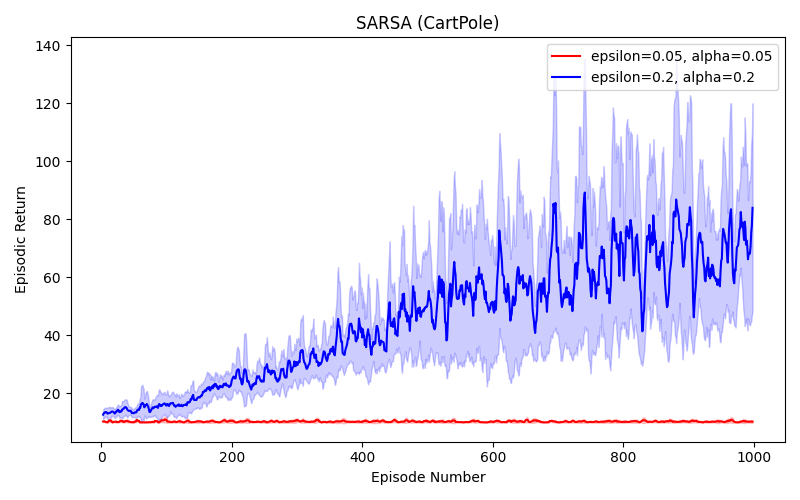
\includegraphics[width=\textwidth]{../plots/sarsa_0.05_0.05vs0.2_0.2.png}
					\caption{$\alpha = 0.05$}
				\end{subfigure}
				\hfill
				\begin{subfigure}[h]{0.3\textwidth}
					\centering
					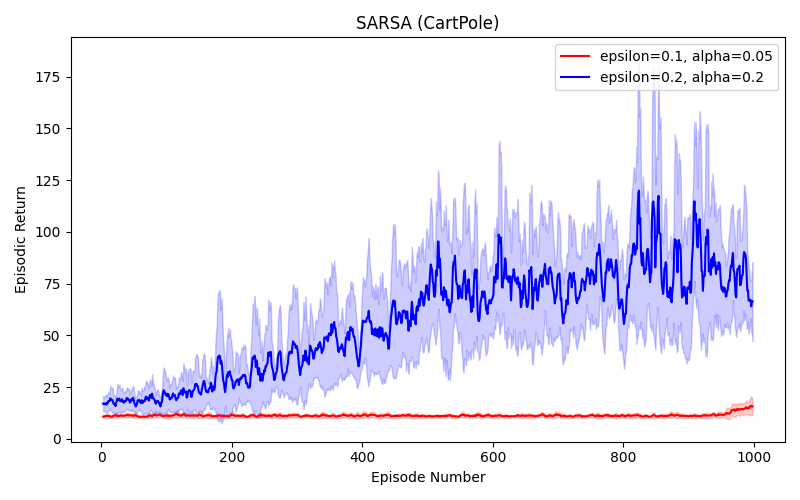
\includegraphics[width=\textwidth]{../plots/sarsa_0.05_0.1vs0.2_0.2.png}
					\caption{$\epsilon = 0.1$}
				\end{subfigure}
				\hfill
				\begin{subfigure}[h]{0.3\textwidth}
					\centering
					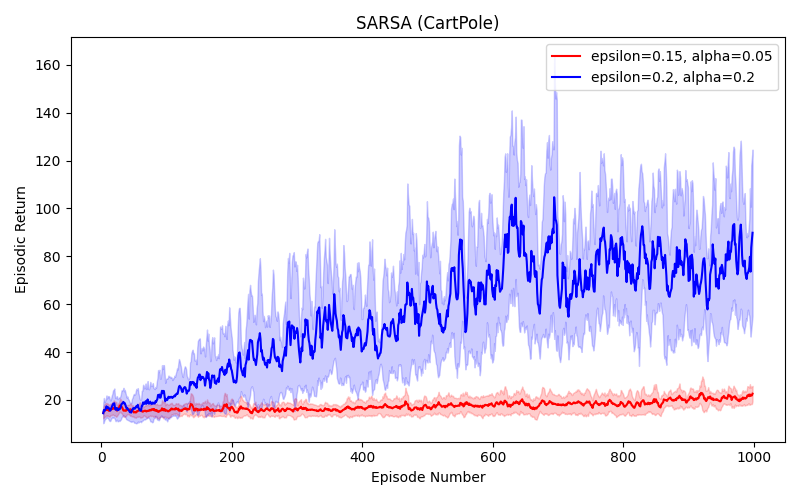
\includegraphics[width=\textwidth]{../plots/sarsa_0.05_0.15vs0.2_0.2.png}
					\caption{$\epsilon = 0.15$}
				\end{subfigure}
				
				\vspace{0.1cm} % Space between rows
				
				% Row 2
				\begin{subfigure}[h]{0.3\textwidth}
					\centering
					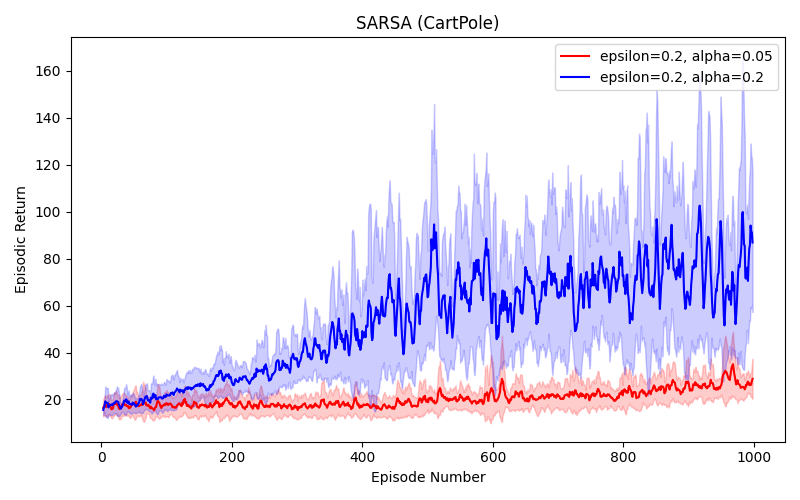
\includegraphics[width=\textwidth]{../plots/sarsa_0.05_0.2vs0.2_0.2.png}
					\caption{$\epsilon = 0.2$}
				\end{subfigure}
				\hfill
				\begin{subfigure}[h]{0.3\textwidth}
					\centering
					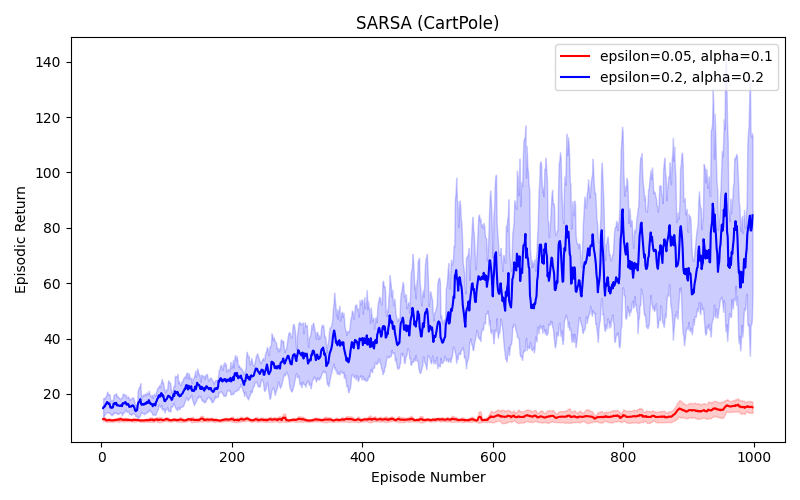
\includegraphics[width=\textwidth]{../plots/sarsa_0.1_0.05vs0.2_0.2.png}
					\caption{$\epsilon = 0.25$}
				\end{subfigure}
				\hfill
				\begin{subfigure}[h]{0.3\textwidth}
					\centering
					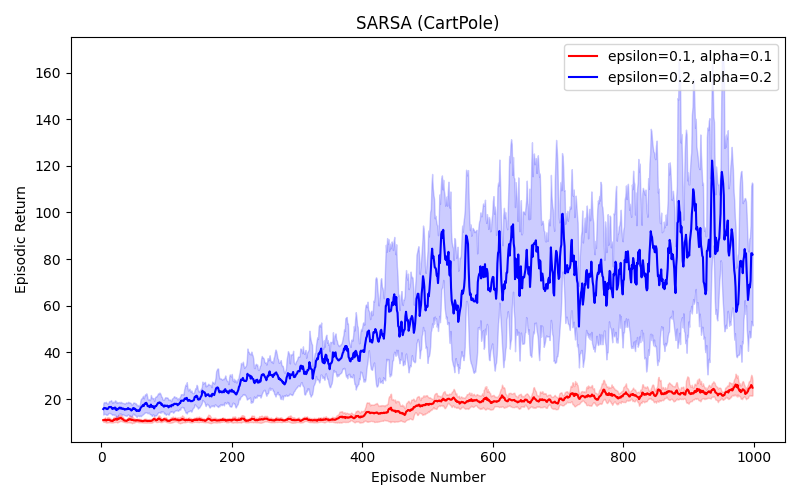
\includegraphics[width=\textwidth]{../plots/sarsa_0.1_0.1vs0.2_0.2.png}
					\caption{$\epsilon = 0.3$}
				\end{subfigure}
				
				\vspace{0.1cm}
				
				% Row 3
				\begin{subfigure}[h]{0.3\textwidth}
					\centering
					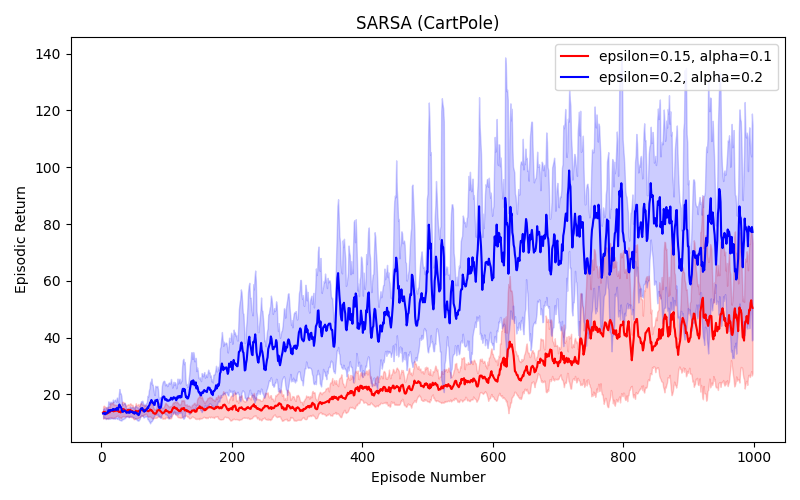
\includegraphics[width=\textwidth]{../plots/sarsa_0.1_0.15vs0.2_0.2.png}
					\caption{$\epsilon = 0.35$}
				\end{subfigure}
				\hfill
				\begin{subfigure}[h]{0.3\textwidth}
					\centering
					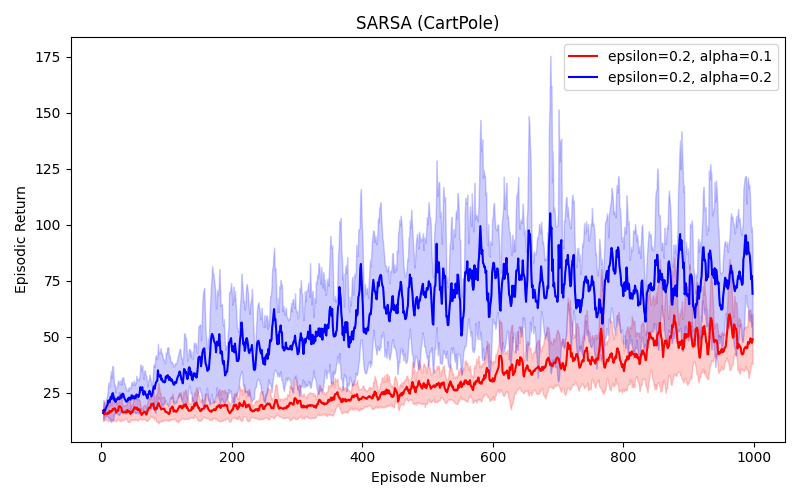
\includegraphics[width=\textwidth]{../plots/sarsa_0.1_0.2vs0.2_0.2.png}
					\caption{$\epsilon = 0.4$}
				\end{subfigure}
				\hfill
				\begin{subfigure}[h]{0.3\textwidth}
					\centering
					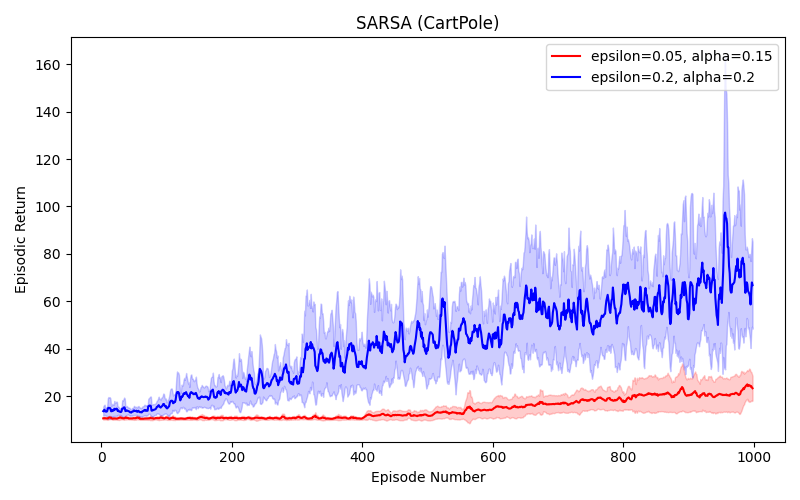
\includegraphics[width=\textwidth]{../plots/sarsa_0.15_0.05vs0.2_0.2.png}
					\caption{$\epsilon = 0.45$}
				\end{subfigure}
				
				\vspace{0.1cm}
				
				% Row 4
				\begin{subfigure}[h]{0.3\textwidth}
					\centering
					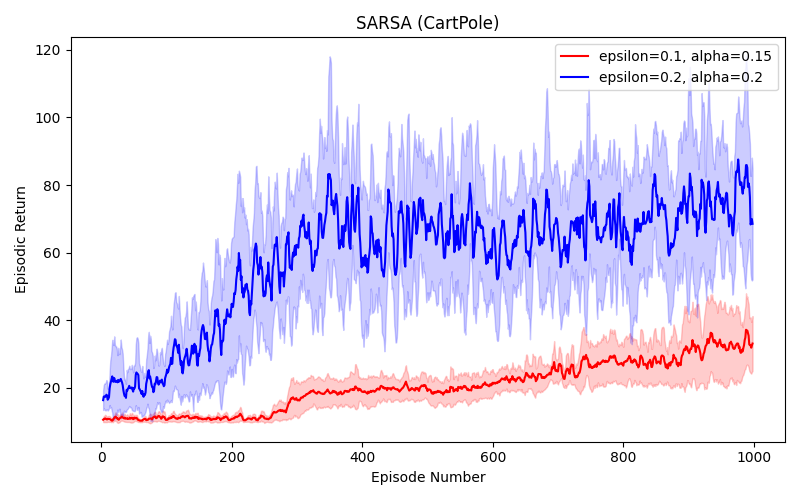
\includegraphics[width=\textwidth]{../plots/sarsa_0.15_0.1vs0.2_0.2.png}
					\caption{$\epsilon = 0.5$}
				\end{subfigure}
				\hfill
				\begin{subfigure}[h]{0.3\textwidth}
					\centering
					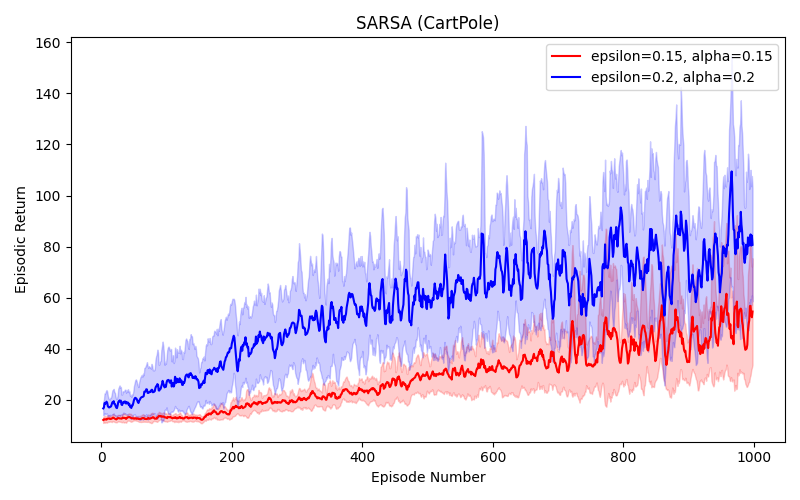
\includegraphics[width=\textwidth]{../plots/sarsa_0.15_0.15vs0.2_0.2.png}
					\caption{$\epsilon = 0.55$}
				\end{subfigure}
				\hfill
				\begin{subfigure}[h]{0.3\textwidth}
					\centering
					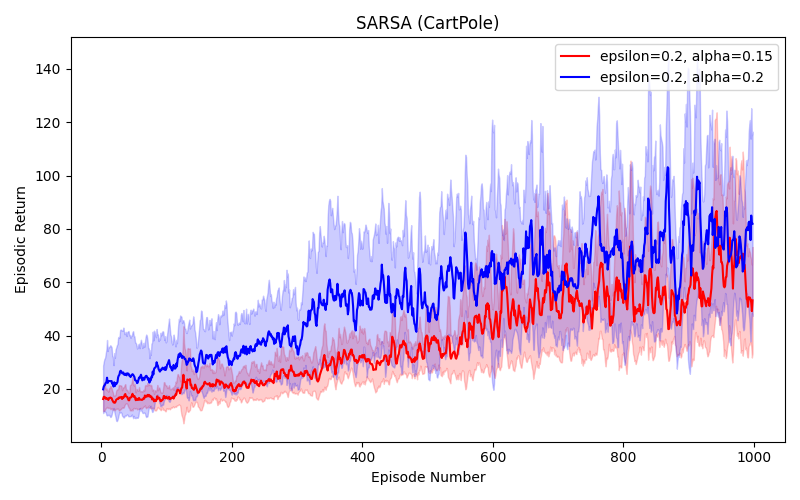
\includegraphics[width=\textwidth]{../plots/sarsa_0.15_0.2vs0.2_0.2.png}
					\caption{$\epsilon = 0.6$}
				\end{subfigure}
				
				\vspace{0.1cm}
				
				% Row 5
				\begin{subfigure}[h]{0.3\textwidth}
					\centering
					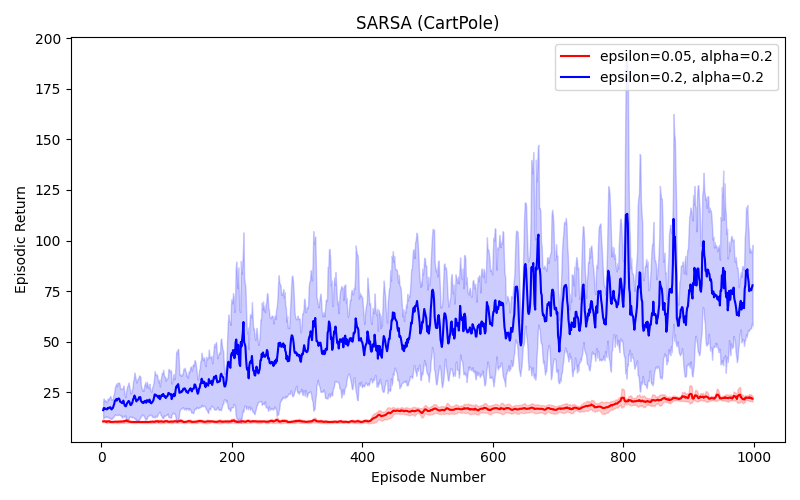
\includegraphics[width=\textwidth]{../plots/sarsa_0.2_0.05vs0.2_0.2.png}
					\caption{$\epsilon = 0.65$}
				\end{subfigure}
				\hfill
				\begin{subfigure}[h]{0.3\textwidth}
					\centering
					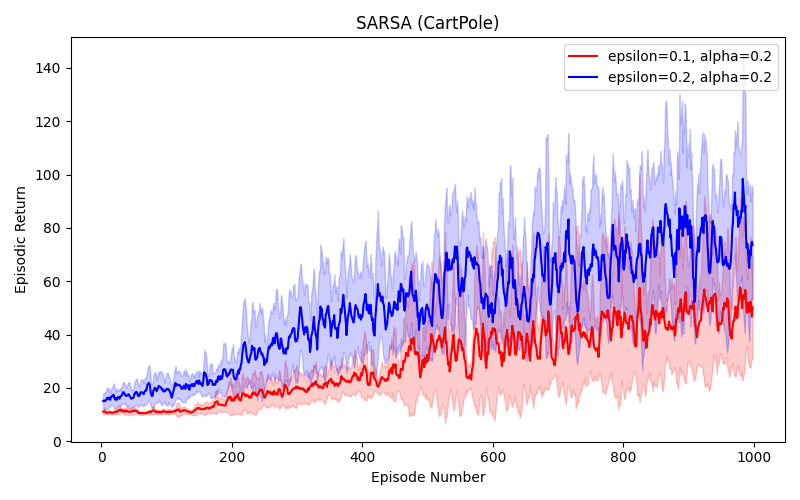
\includegraphics[width=\textwidth]{../plots/sarsa_0.2_0.1vs0.2_0.2.png}
					\caption{$\epsilon = 0.7$}
				\end{subfigure}
				\hfill
				\begin{subfigure}[h]{0.3\textwidth}
					\centering
					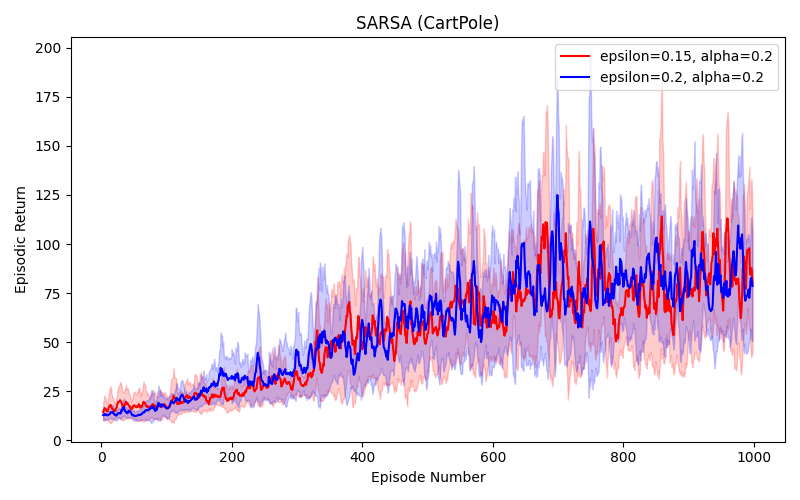
\includegraphics[width=\textwidth]{../plots/sarsa_0.2_0.15vs0.2_0.2.png}
					\caption{$\epsilon = 0.75$}
				\end{subfigure}
				
				\caption{Phase portraits for different values of $\epsilon$}
				\label{fig:phase_portraits}
			\end{figure}
\end{document}